% Chapter Template

\chapter{Ensayos y resultados} % Main chapter title
En este capitulo se explica las pruebas realizadas al hardware, firmware , controladores y a la plataforma IoT a lo largo del trabajo.
\label{Chapter4} % Change X to a consecutive number; for referencing this chapter elsewhere, use \ref{ChapterX}

%----------------------------------------------------------------------------------------
%	SECTION 1
%----------------------------------------------------------------------------------------

\section{Pruebas Unitarias}
Para el desarrollo de los drivers del modulo BG96 y el sensor AHT10 se utilizo la metodologia de desarrollo TDD. Esto implica que se escribieron pruebas unitarias para los drivers utilizando ceedling herramienta para el desarrollado de pruebas automaticas.En las figuras \ref{cod:codigo test driver AHT10} y \ref{cod:codigo test driver bg96} se pueden ver algunas pruebas para los drivers desarrollados.
\begin{lstlisting}[label=cod:codigo test driver AHT10,caption=Tests del driver sensor AHT10.] 
//Prueba para obtener el estado del sensor AHT10
void test_estado_del_sensor(void)
{
  uint8_t buffer[1]={0};
  uint8_t data=0;
  read_I2C_STM32L432_port_ExpectAndReturn(AHT10_ADDRESS_SLAVE,buffer,1,AHT10_OK);
  read_I2C_STM32L432_port_ReturnThruPtr_buffer(&data);
  TEST_ASSERT_EQUAL(SENSOR_IDLE,aht10_get_status(&aht10config));
  
  data=255;
  read_I2C_STM32L432_port_ExpectAndReturn(AHT10_ADDRESS_SLAVE,buffer,1,AHT10_OK);
  read_I2C_STM32L432_port_ReturnThruPtr_buffer(&data);
  TEST_ASSERT_EQUAL(SENSOR_BUSY,aht10_get_status(&aht10config));
  
  read_I2C_STM32L432_port_ExpectAndReturn(AHT10_ADDRESS_SLAVE,buffer,1,AHT10_ERROR);
  TEST_ASSERT_EQUAL(SENSOR_BUSY,aht10_get_status(&aht10config)); 
}

//Prueba para obtener el valor de la humedad que lee el sensor AHT10
void test_obtener_humedad(void)
{
  uint8_t bufferRead[6]={0};
  uint8_t humedad=0;
  uint8_t cmd[3] = {AHT10_CMD_TRIGGER_MEASUREMENT,AHT10_CMD_DATO_0,AHT10_CMD_DATO_1};
  uint8_t buffer[1]={0};
  write_I2C_STM32L432_port_ExpectAndReturn(AHT10_ADDRESS_SLAVE,cmd,3,AHT10_OK);
  delay_STM32L432_port_Expect(AHT10_DELAY_LAUNCH_MEASUREMENT);
  read_I2C_STM32L432_port_ExpectAndReturn(AHT10_ADDRESS_SLAVE,buffer,1,AHT10_OK);
  write_I2C_STM32L432_port_ExpectAndReturn(AHT10_ADDRESS_SLAVE,cmd,3,AHT10_OK);
  delay_STM32L432_port_Expect(AHT10_DELAY_LAUNCH_MEASUREMENT); 
  read_I2C_STM32L432_port_ExpectAndReturn(AHT10_ADDRESS_SLAVE,bufferRead,6,AHT10_OK);
  TEST_ASSERT_EQUAL(AHT10_OK,aht10_get_humedity(&aht10config,&humedad));
  TEST_ASSERT_EQUAL(0,humedad);

  write_I2C_STM32L432_port_ExpectAndReturn(AHT10_ADDRESS_SLAVE,cmd,3,AHT10_ERROR);
  TEST_ASSERT_EQUAL(AHT10_ERROR,aht10_get_humedity(&aht10config,&humedad));

  write_I2C_STM32L432_port_ExpectAndReturn(AHT10_ADDRESS_SLAVE,cmd,3,AHT10_OK);
  delay_STM32L432_port_Expect(AHT10_DELAY_LAUNCH_MEASUREMENT);
  read_I2C_STM32L432_port_ExpectAndReturn(AHT10_ADDRESS_SLAVE,buffer,1,AHT10_OK);
  write_I2C_STM32L432_port_ExpectAndReturn(AHT10_ADDRESS_SLAVE,cmd,3,AHT10_OK);
  delay_STM32L432_port_Expect(AHT10_DELAY_LAUNCH_MEASUREMENT); 
  read_I2C_STM32L432_port_ExpectAndReturn(AHT10_ADDRESS_SLAVE,bufferRead,6,AHT10_ERROR);
  TEST_ASSERT_EQUAL(AHT10_ERROR,aht10_get_humedity(&aht10config,&humedad));
}
\end{lstlisting}

\begin{lstlisting}[label=cod:codigo test driver bg96,caption=Tests del driver modulo bg96.] 
//Prueba para la funcion para obtener el estado en el que se encuentra el modulo bg96
void test_get_status_modem(void)
{
  char buffer_resp[20]={0};
  send_data_ExpectAndReturn(CMD_BG96_STATUS_MODEM,RS_BG96_OK,buffer_resp,1000,FT_BG96_OK);
  TEST_ASSERT_EQUAL(FT_BG96_OK,get_status_modem(&config_module));

  send_data_ExpectAndReturn(CMD_BG96_STATUS_MODEM,RS_BG96_OK,buffer_resp,1000,FT_BG96_ERROR);
  TEST_ASSERT_EQUAL(FT_BG96_ERROR,get_status_modem(&config_module));
}

//Prueba de la funcion para mandar sms  
void test_send_sms_bg96(void)
{
  char buffer_resp[30]={0};
  send_data_ExpectAndReturn("AT+CMGS=\"72950576\"\r",RS_BG96_SIGNAL,buffer_resp,12000,FT_BG96_OK);
  send_data_ExpectAndReturn("HOLA\x1a\r",RS_BG96_OK,buffer_resp,12000,FT_BG96_OK);
  TEST_ASSERT_EQUAL(FT_BG96_OK,send_sms_bg96(&config_module,"72950576","HOLA"));

  send_data_ExpectAndReturn("AT+CMGS=\"72950576\"\r",RS_BG96_SIGNAL,buffer_resp,12000,FT_BG96_ERROR);
  TEST_ASSERT_EQUAL(FT_BG96_ERROR,send_sms_bg96(&config_module,"72950576","HOLA"));

  send_data_ExpectAndReturn("AT+CMGS=\"72950576\"\r",RS_BG96_SIGNAL,buffer_resp,12000,FT_BG96_OK);
  send_data_ExpectAndReturn("HOLA\x1a\r",RS_BG96_OK,buffer_resp,12000,FT_BG96_ERROR);
  TEST_ASSERT_EQUAL(FT_BG96_ERROR,send_sms_bg96(&config_module,"72950576","HOLA"));
}

//Prueba de la funcion para publicar mensajes al broker mqtt
void test_publish_message(void)
{
  char buffer_resp[30]={0};
  char topic[19]="/v1.6/devices/demo";
  char data[25]="{\"demo\":10,\"humedad\":60}";
  send_data_ExpectAndReturn("AT+QMTPUB=0,0,0,0,\"/v1.6/devices/demo\"\r",RS_BG96_SIGNAL,buffer_resp,3000,FT_BG96_OK);
  send_data_ExpectAndReturn("{\"demo\":10,\"humedad\":60}\x1a\r",RS_BG96_CERO,buffer_resp,15000,FT_BG96_OK);
  TEST_ASSERT_EQUAL(FT_BG96_OK,publish_message(&config_module,topic,data));

  send_data_ExpectAndReturn("AT+QMTPUB=0,0,0,0,\"/v1.6/devices/demo\"\r",RS_BG96_SIGNAL,buffer_resp,3000,FT_BG96_ERROR);
  TEST_ASSERT_EQUAL(FT_BG96_ERROR,publish_message(&config_module,topic,data));

  send_data_ExpectAndReturn("AT+QMTPUB=0,0,0,0,\"/v1.6/devices/demo\"\r",RS_BG96_SIGNAL,buffer_resp,3000,FT_BG96_OK);
  send_data_ExpectAndReturn("{\"demo\":10,\"humedad\":60}\x1a\r",RS_BG96_CERO,buffer_resp,15000,FT_BG96_ERROR);
  TEST_ASSERT_EQUAL(FT_BG96_ERROR,publish_message(&config_module,topic,data));
}
\end{lstlisting}

Una forma cuantitativa de evaluar estas pruebas son los informes de cobertura generados por ceedling.

En la figura \ref{fig:Cobertura aht10} se puede observar el informe de cobertura del driver aht10, donde se puede apreciar que las pruebas ejecutan el 100\% de las lineas de codigo escritas y explora el 100\% de las conbinaciones en los saltos de condicionales.

En la figura \ref{fig:Cobertura BG96} tambien se observa el informe de cobertura del dirver de BG96, con 98.4\% de lineas ejecutadas y explora mas del 98.3\% de combinaciones posibles. 

\begin{figure}[h!]
    \centering
      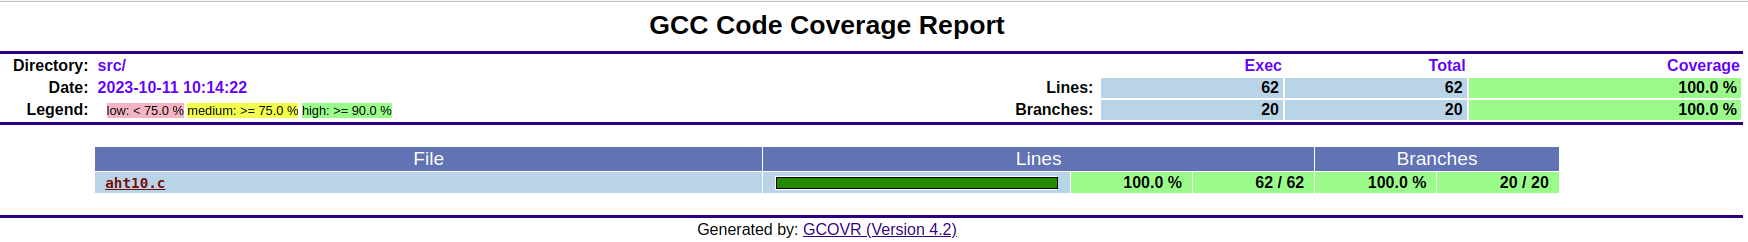
\includegraphics[width=\linewidth, height=6cm]{./Figures/cobertura_aht10.png}
    \caption{Informe de cobertura driver aht10.}
      \label{fig:Cobertura aht10}
  \end{figure}

\begin{figure}[htbp!]
    \centering
      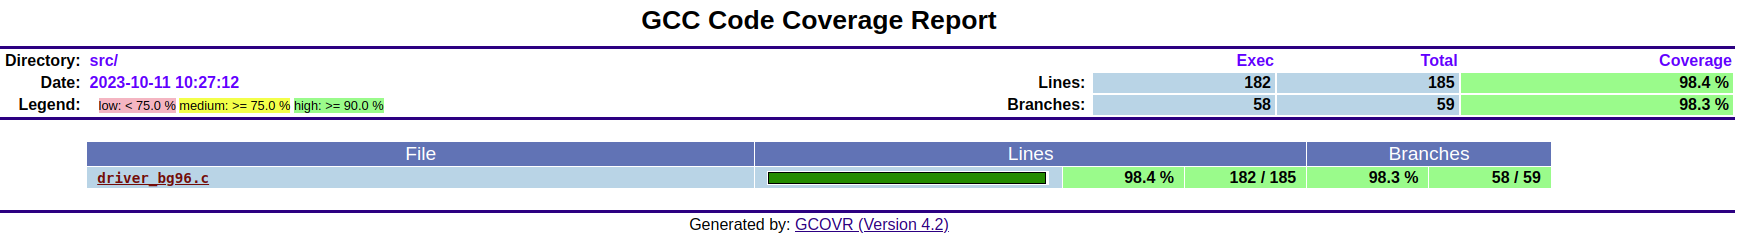
\includegraphics[width=\linewidth, height=6cm]{./Figures/cobertura_bg96.png}
    \caption{Informe de cobertura driver BG96.}
      \label{fig:Cobertura BG96}
\end{figure}
\section{Pruebas De Hardware}
\subsection{Prueba sensor de humedad AHT10}
Para probar el correcto funcionamiento del sensor AHT10 y la correcta comunicacion con el microcontrolador se comprobo la trama I2C con un analizador logico,
en la figura \ref{fig:write aht10} podemos ver la trama capturada cuando queremos escribir en un registro del sensor y en la figura \ref{fig:read aht10} tenemos la trama cuando leemos los registros del sensor donde se obtiene 6 bytes en los que se encuantra la informacion de la humedad y la temperatura. 

\begin{figure}[h!]
  \centering
    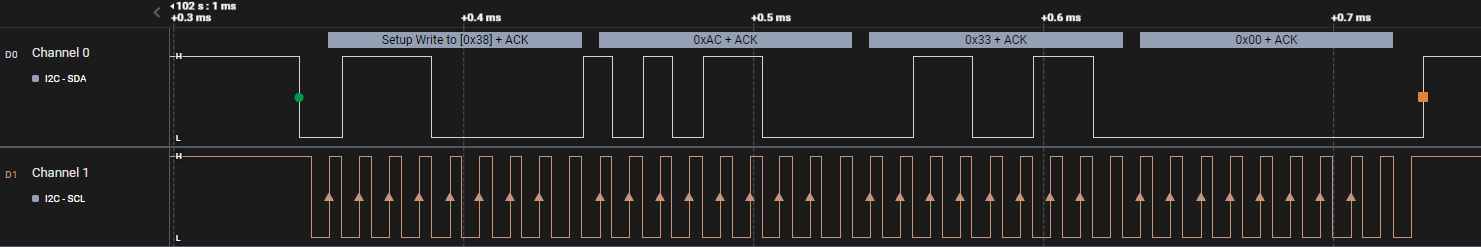
\includegraphics[width=\linewidth, height=4.5cm]{./Figures/write_i2c.png}
  \caption{Trama de escritura al sensor AHT10.}
    \label{fig:write aht10}
\end{figure}

\begin{figure}[h!]
  \centering
    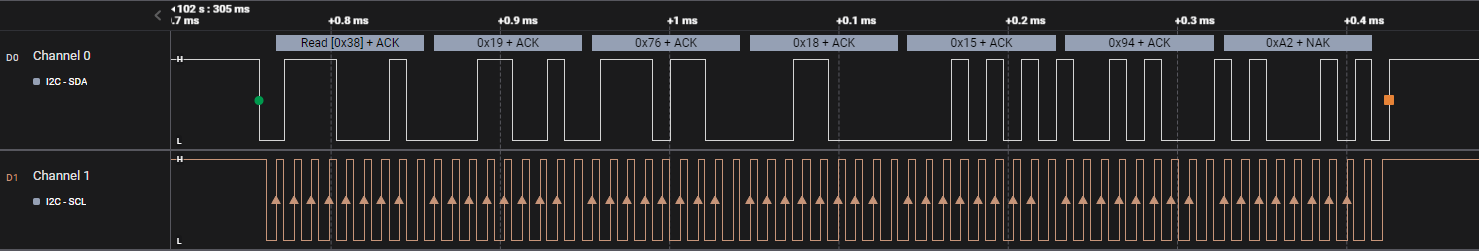
\includegraphics[width=\linewidth, height=4.5cm]{./Figures/read_i2c..png}
  \caption{Trama de lectura del sensor AHT10.}
    \label{fig:read aht10}
\end{figure}

\subsection{Pruebas comunicacion por UART con modulo de comunicacion BG96}

Para probar la comunicacion del microcontrolador con el modulo por UART se utlizo un analizador logico que nos permite los comandos que envia el microcontrolador y la respuestas del modulo a estos comandos.
En la figura podemos ver esta comunicacion bidirecional por puerto AURT.

\begin{figure}[h!]
  \centering
    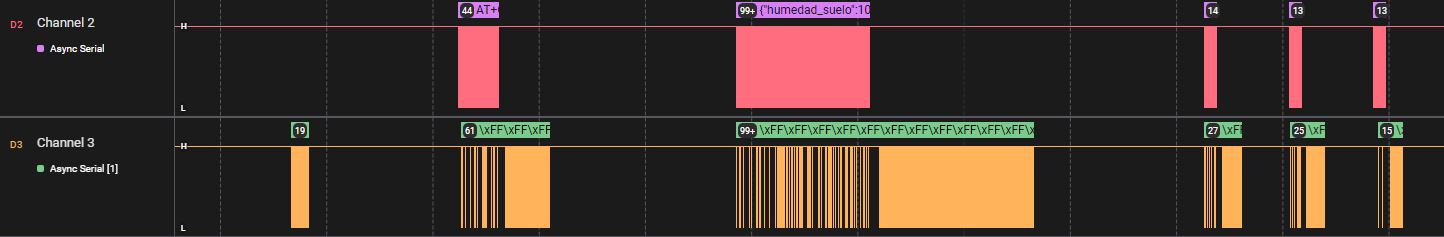
\includegraphics[width=\linewidth, height=4cm]{./Figures/trama_uart4.png}
  \caption{Informe de cobertura driver aht10.}
    \label{fig:trama uart}
\end{figure}

\begin{figure}[h!]
  \centering
    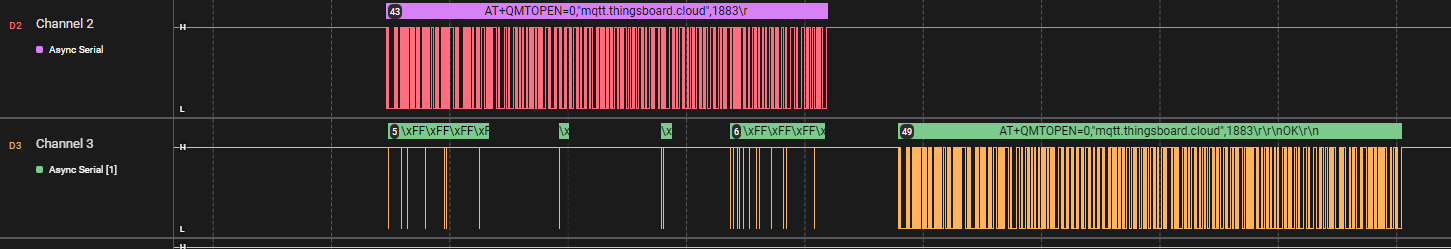
\includegraphics[width=\linewidth, height=4cm]{./Figures/trama_uart1.png}
  \caption{Informe de cobertura driver aht10.}
    \label{fig:trama uart1}
\end{figure}

\subsection{Pruebas bajo consumo }
Al se un dispositivo que funcionara a bateria lo que busca el firmware consumir lo menos posible, lo que se hizo fue hacer hacer la lectura de los sensores y enviar los datos cada 15min y el el tiempo restante mandar el microcontrolador a bajo consumo 
En la figura podemos ver el consumo del sistema normalmente y eb bajo consumo.


\subsection{Pruebas de alimetaccion del modulorealzado}

\clearpage 
\section{Pruebas del firmware}
\subsection{Pruebas de conexion con broker mqtt}
Una de las tareas mas importante del firmware es la del manejo del servidor,para verficar el correcto funcionamiento de esta tarea tenemos que ver la secuencia de comandos que son mandados del microcontroaldor al modulo de comunicion por el puerto UART.

En la figura podemos observar toda la secuencia de envio de datos a la plataforma Iot, primeramente el modulo optine un apn del proveedor del red, luego

\begin{figure}[h]
  \centering
    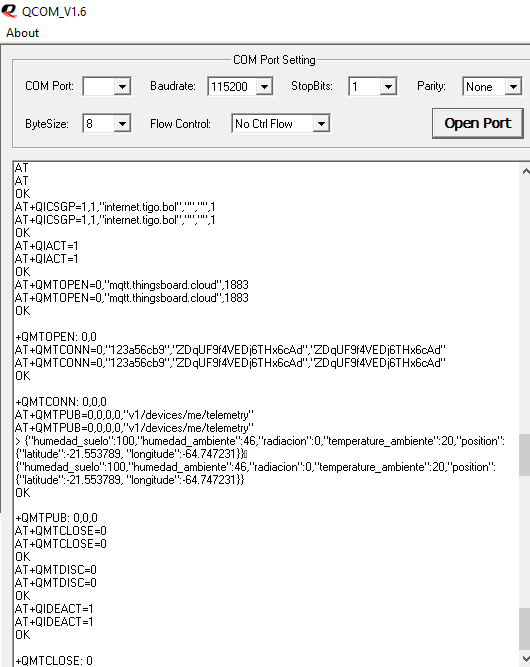
\includegraphics[width=8cm, height=12cm]{./Figures/Qcom_enviodedatos.png}
  \caption{Informe de cobertura driver aht10.}
    \label{fig:conexion broker}
\end{figure}

\subsection{Pruebas de alarmas}
El objetivo de esta prueba es comprobar el buen funcionamiento de las alarmas del sistema.
Cuando la humedad del suelo baja por debajo del rango permitido por el sistema, el firmware manda un sms al usuario con la alarma ocurrida.En la figura podemos ver que la humedad bajo de 5\% y en la figura se resibio el sms.

\begin{figure}[h!]
  \centering
    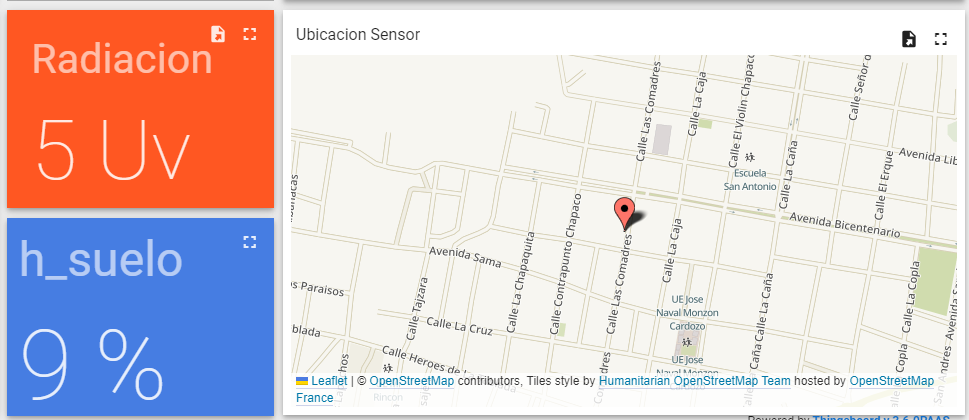
\includegraphics[width=\linewidth, height=7cm]{./Figures/humedad_menor2.png}
  \caption{Informe de cobertura driver aht10.}
    \label{fig:humedad menor}
\end{figure}

\begin{figure}[h!]
  \centering
    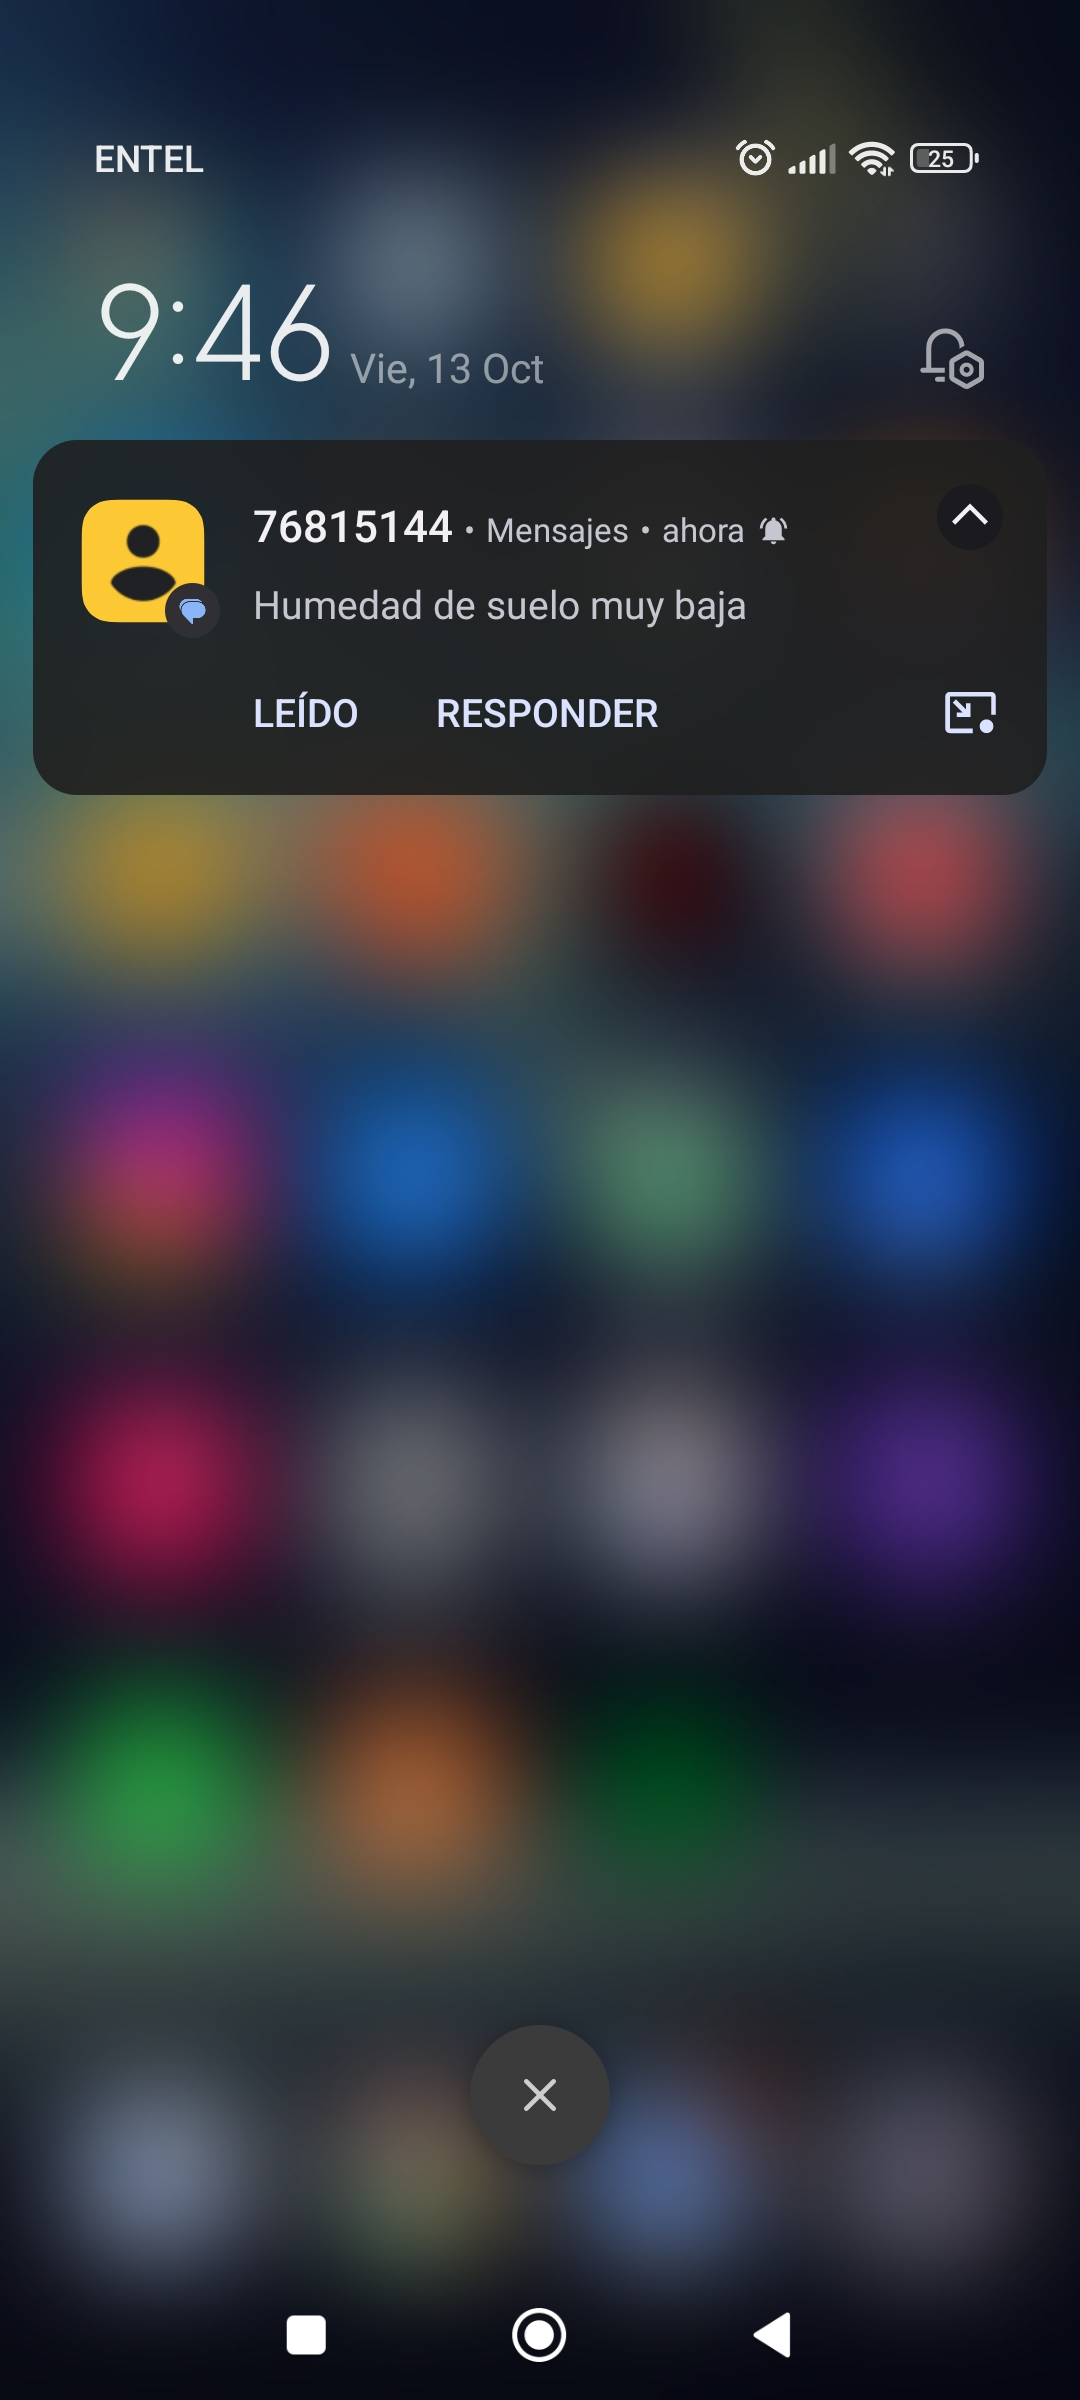
\includegraphics[width=8cm, height=12cm]{./Figures/sms_alarma.jpg}
  \caption{Informe de cobertura driver aht10.}
    \label{fig:sms alarma}
\end{figure}
\clearpage 
\section{Pruebas de la plataforma IoT}
\subsection{Pruebas de inyeccion de mensajes}
El objetivo de las pruebas de la plataforma IoT es evaluar la llegada de los mensajes por protocolo MQTT.
Para su realizacion se utilizo la aplicación de linea de comandos de mosquitto.
Para realizar el envio de datos a broker MQTT, se utiliza el cliente MQTT de mosquitto utilizando el comando que se muestra en la figura .

\begin{figure}[h!]
  \centering
    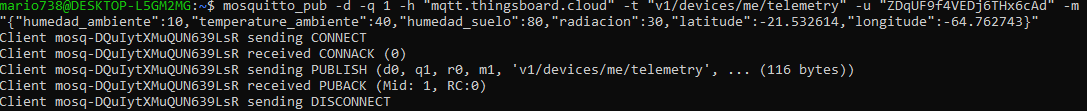
\includegraphics[width=\linewidth, height=3cm]{./Figures/mosquito_enviodatos.png}
  \caption{Informe de cobertura driver aht10.}
    \label{fig:mosquitto pub}
\end{figure}

Donde:

Posterior a ejecutar el comando podemos ver lo que se es es conectar el servidor , enviar 

Para comprobar la llegada de los valores al broker de ThingsBoard tenemos que ir a la seccion dispositivos, seleccionar el dispositivo al que se le envio los datos y entrar a la pestana de ultima telemetria, en la figura podemos ver que los datos llegaron correctamente.
\begin{figure}[h!]
  \centering
    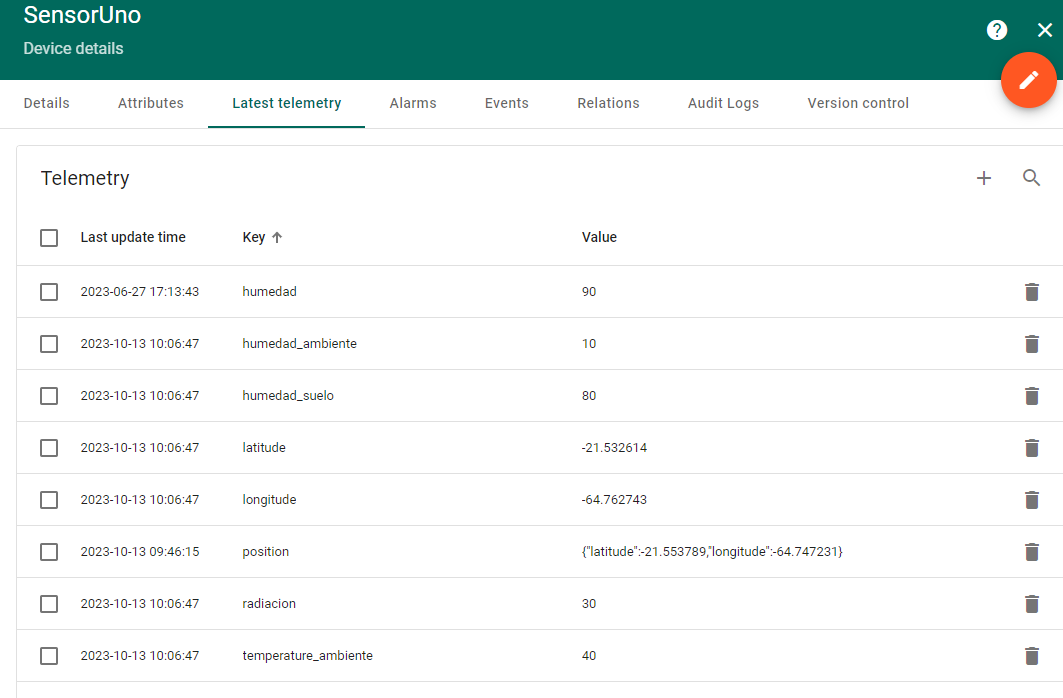
\includegraphics[width=7cm, height=10cmcm]{./Figures/tb_recepcion.png}
  \caption{Informe de cobertura driver aht10.}
    \label{fig:tb recepcion}
\end{figure}
\subsection{Pruebas notificaciones en thingsboard}
Cuando la temperatura ambiente supera los 45 grados la plataforma nos notifica que existe alarma 
\begin{figure}[h!]
  \centering
    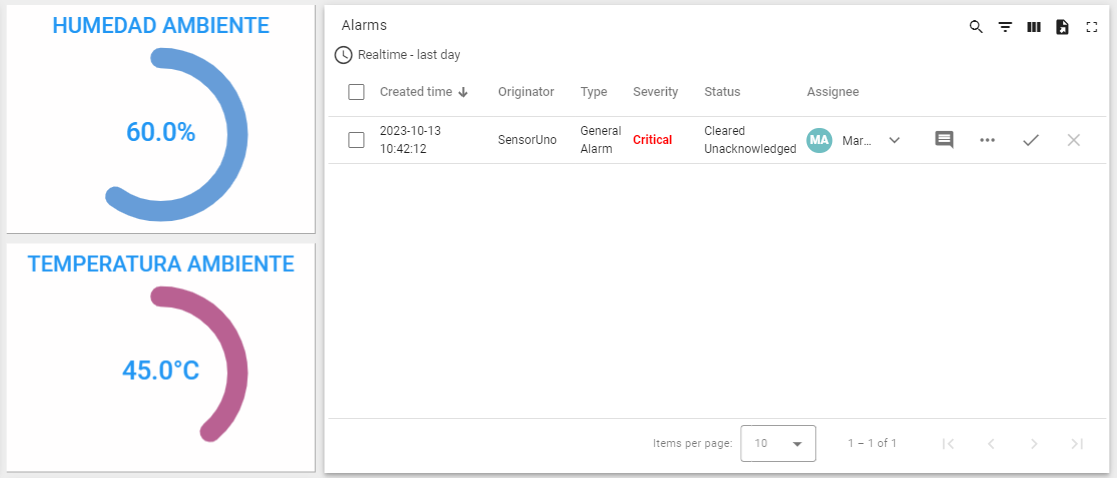
\includegraphics[width=\linewidth, height=9cm]{./Figures/alarmas_tb.png}
  \caption{Informe de cobertura driver aht10.}
    \label{fig:alarmas tb}
\end{figure}

\subsection{Pruebas de la witget}

\begin{figure}[h!]
  \centering
    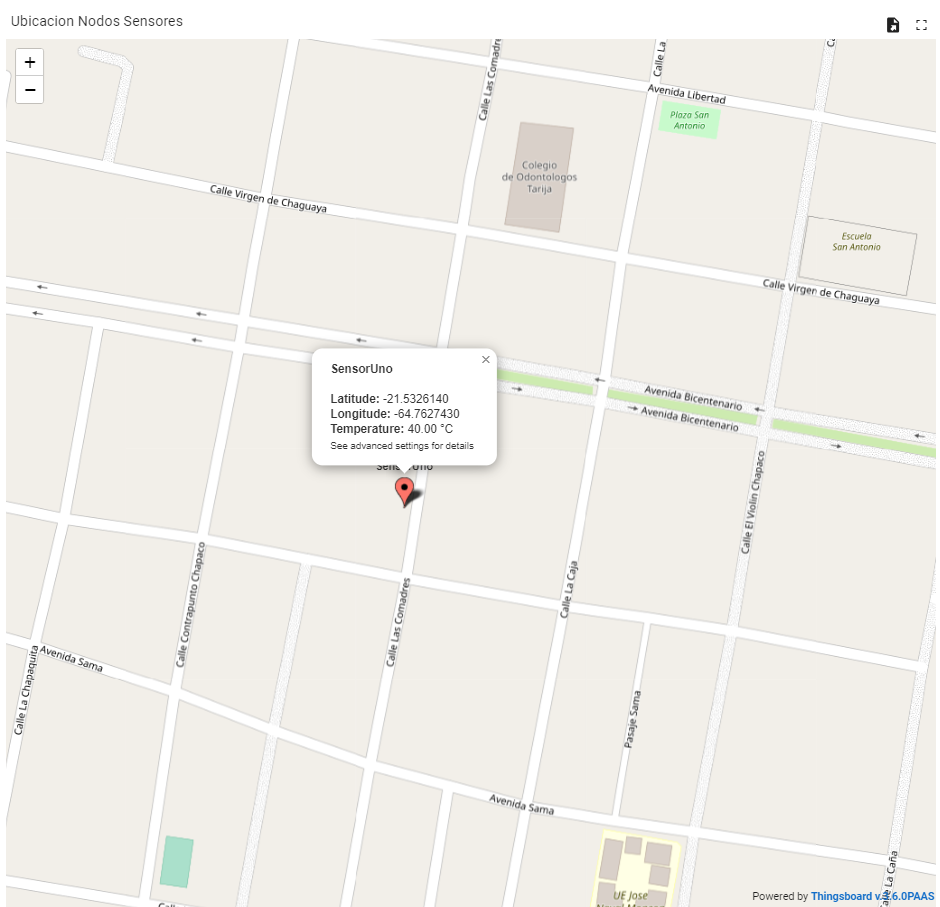
\includegraphics[width=\linewidth, height=9cm]{./Figures/map.png}
  \caption{Informe de cobertura driver aht10.}
    \label{fig:map thingsboard}
\end{figure}


\section{Pruebas Funcionales}

\label{sec:pruebasHW}

